\chapter{Codes et Algèbre de Boole}
\section{Code}
Pour pouvoir, en binaire, représenter les chiffres de 0 à 9, il nous faut au minimum 4 bits ($\log_2 10$). Donc, nous perdons 6 codes du à l'arrondissement à 4 bits (1010, 1011, 1100, 1101, 1101 et 1111). En octal et hexadécimal, c'est plus pratique car il n'y a pas de perte du à l'arrondissement ($\log_2 8=3$ et $\log_2 16=4$).Il y a donc, d'autres façons de coder en fonction de l'utilisation qu'on en fait. On en distingue 3 classes: 
\begin{enumerate}
	\item 	Codes pondérés (\textit{weighted codes})
	\begin{itemize}
		\item 8421 \textit{Binary coded Decimal} (BCD) où chaque chiffre est codé séparément
		\item Codes auto-complémentaires
		\begin{itemize}
			\item 2421 Code
			\item Code excédent 3 (Excess 3)
		\end{itemize}
	\end{itemize}
	\item Codes non-pondérés
	\begin{itemize}
		\item Code Gray (code cyclique)
		\item \textit{American Standard Code for Information Interchage} (code ASCII)
	\end{itemize}
	\item Code détecteurs d'erreur
\end{enumerate}
\subsection{Codes pondérés}
Voici une table pour bien comprendre comment fonctionnent les codes auto-complémentaires (le $-$ de $-3$ correspond au chiffre négatif)
\begin{table}[H]
	\centering
	\begin{tabular}{c|c|c|c}
		Décimal & 8421 (BCD) & 2421 & 642-3 \\
		\hline
		0 & 0000 & 0000 & 0000\\
		\hline
		1 & 0001 & 0001 & 0101\\
		\hline
		2 & 0010 & 0010 & 0010\\
		\hline
		3 & 0011 & 0011 & 1001\\
		\hline
		4 & 0100 & 0100 & 0100\\
		\hline
		5 & 0101 & 1011 & 1011\\
		\hline
		6 & 0110 & 1100 & 0110\\
		\hline
		7 & 0111 & 1101 & 1101\\
		\hline
		8 & 1000 & 1110 & 1010\\
		\hline
		9 & 1001 & 1111 & 1111		
	\end{tabular}
	\caption{Code auto-complémentaire}
\end{table}
\subsubsection{Addition en BCD}
L'addition en BCD est simple, on additionne par 4 bits (chaque chiffre composant la base 10). Si le chiffre est $\geq 10$, on ajoute $+6\,(0110)_2$ car cela correspond à un report de 10 en binaire. En effet, regroupé par 4 correspond à de l'hexadécimal, du coup, pour passer de 10 à 0, il faut ajouter 6 ($A\overset{+1}{\rightarrow}B\overset{+1}{\rightarrow}\dots\overset{+1}{\rightarrow}F\overset{+1}{\rightarrow}0$). Exemple:
\begin{table}[H]
	\centering
	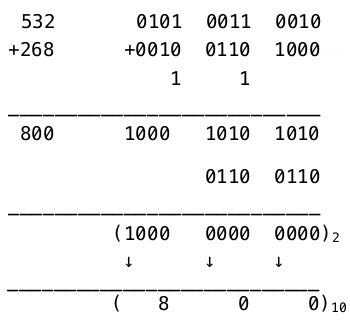
\includegraphics[scale=0.5]{ch2/image1}
\end{table}
\subsection{Codes non-pondérés}
\subsubsection{Code Gray}
Le code Gray est un code suivant le principe de \textit{Look-up Table}, c'est-à-dire que la conversion ne suit pas une règle mais une table de correspondance associant des valeurs. Le principe du Gray est que 2 codes voisins ne diffèrent que par la valeur d'un bit.
\begin{table}[H]
	\centering
	\begin{tabular}{c|c}
		Décimal & Gray \\
		\hline
		0 & 000\\
		 \hline
		1 & 001\\
		 \hline
		2 & 011\\
		 \hline
		3 & 010\\
		 \hline
		4 & 110\\
		 \hline
		5 & 111\\
		 \hline
		6 & 101\\
		 \hline
		7 & 101		 
	\end{tabular}
	\caption{Code Gray}
\end{table}
\subsubsection{Code ASCII}
Le code ASCII est utilisé pour coder les caractères dans des systèmes de traitement numérique, comme les majuscules, les signes de ponctuation et cetera. Le code est basé sur 8 bits, donc 256 possibilités, mais en réalité, on en utilise que 128.
\begin{figure}[H]
	\centering
	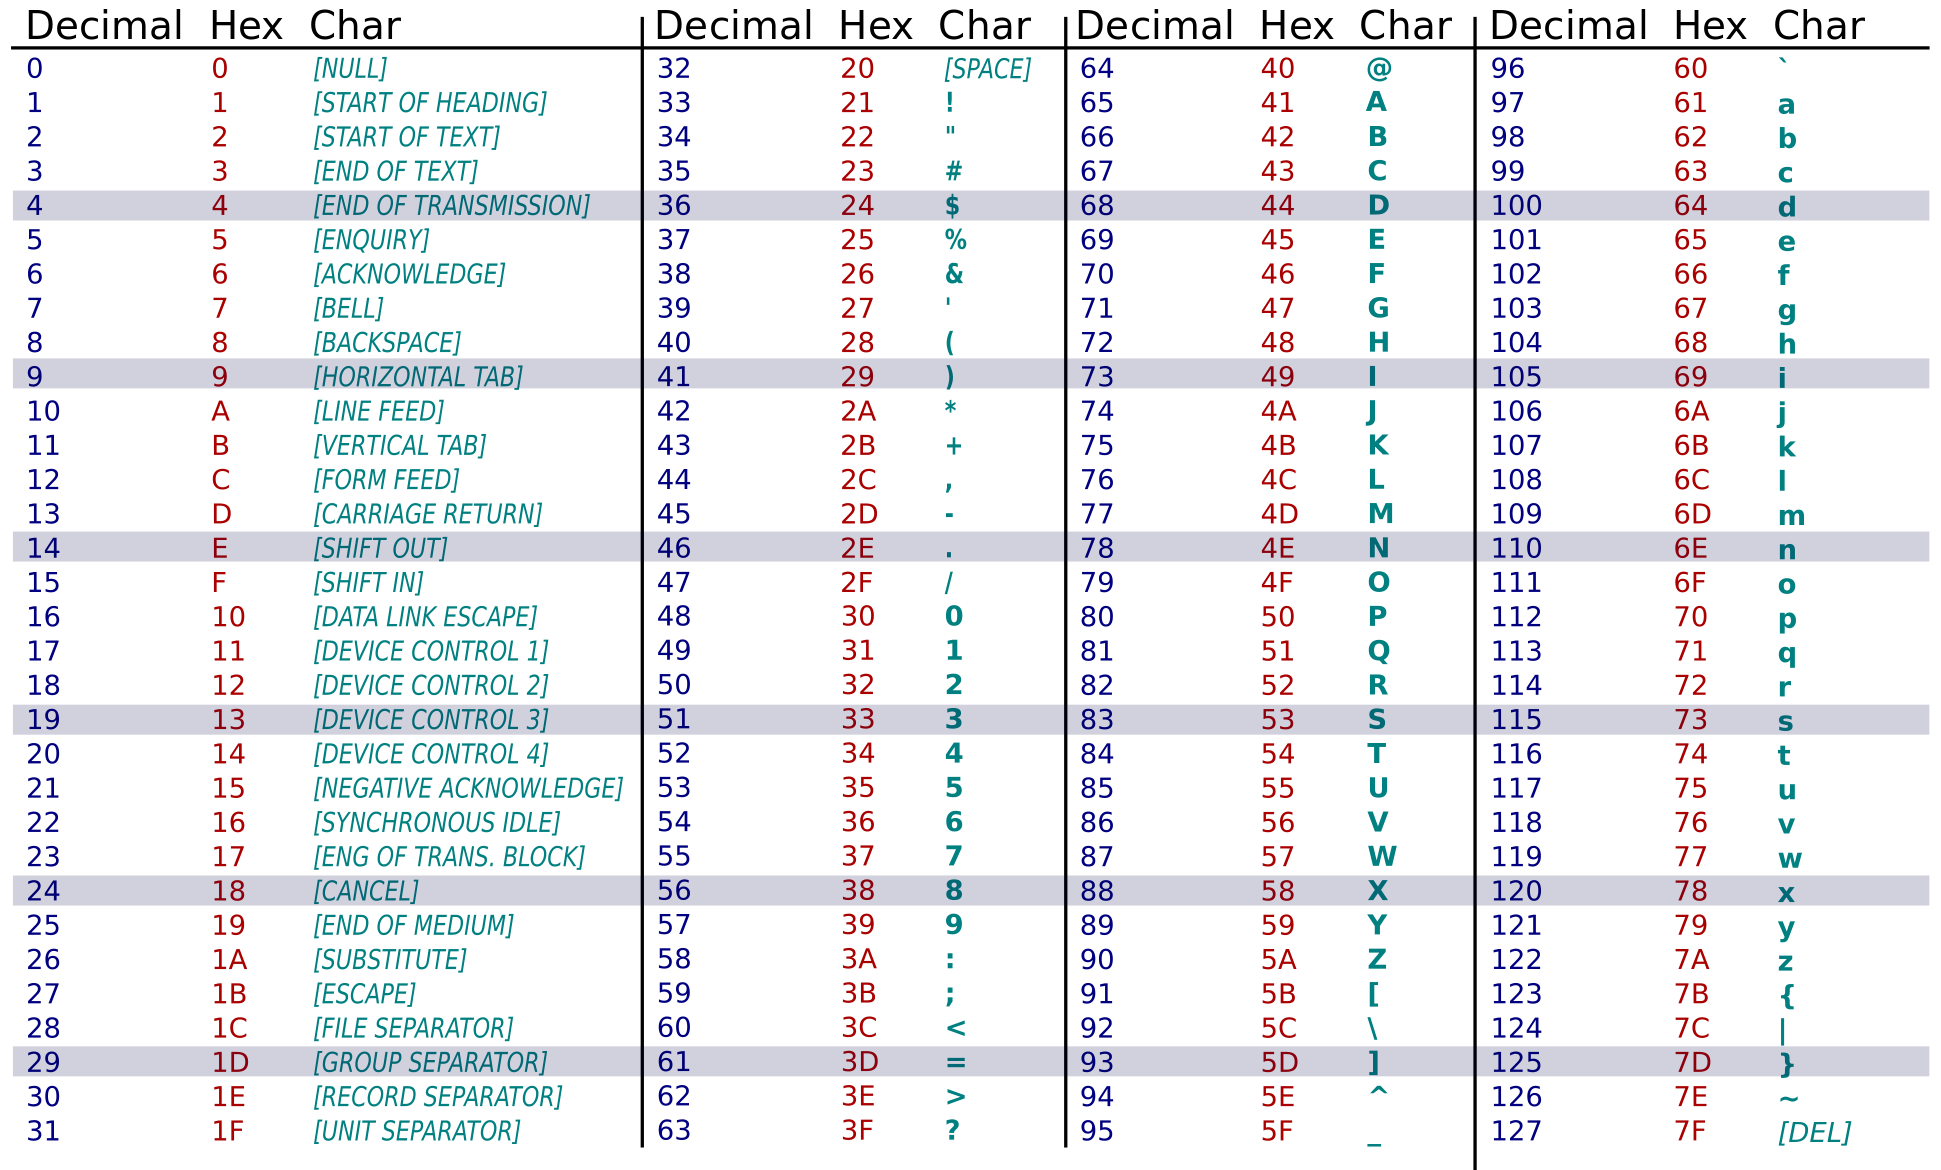
\includegraphics[width=\textwidth]{ch2/image2}
	\caption{Table ASCII}
\end{figure}
\subsection{Codes correcteurs}

\section{Algèbre de Boole}

\section{Fonctions logiques}

\section{Réalisation matérielle}
